%% LyX 2.3.4.2 created this file.  For more info, see http://www.lyx.org/.
%% Do not edit unless you really know what you are doing.
\documentclass[english,dvipsnames,aspectratio=169,handout]{beamer}
\usepackage{mathptmx}
\usepackage{algorithm2e}
\usepackage{eulervm}
\usepackage[T1]{fontenc}
\usepackage[latin9]{inputenc}
\usepackage{babel}
\usepackage{amstext}
\usepackage{amssymb}
\usepackage{graphicx}
\usepackage{ifthen}
\usepackage{xcolor}
\usepackage{xspace}
\usepackage{tikz}
\usetikzlibrary{tikzmark}
\usetikzlibrary{calc}
\usepackage{pgfplots}
%\pgfplotsset{compat=1.17}
\usepackage{booktabs}
\usepackage{xpatch}
\usepackage{multirow}
\usepackage{colortbl}
\usepackage{pgfpages}

%\setbeameroption{show notes on second screen}

\xpatchcmd{\itemize}
  {\def\makelabel}
  {\ifnum\@itemdepth=1\relax
     \setlength\itemsep{2ex}% separation for first level
   \else
     \ifnum\@itemdepth=2\relax
       \setlength\itemsep{1ex}% separation for second level
     \else
       \ifnum\@itemdepth=3\relax
         \setlength\itemsep{0.5ex}% separation for third level
   \fi\fi\fi\def\makelabel
  }
 {}
 {}

\ifx\hypersetup\undefined
  \AtBeginDocument{%
    \hypersetup{unicode=true,pdfusetitle,
 bookmarks=true,bookmarksnumbered=false,bookmarksopen=false,
 breaklinks=false,pdfborder={0 0 0},pdfborderstyle={},backref=false,colorlinks=true,
 allcolors=NYUPurple,urlcolor=LightPurple}
  }
\else
  \hypersetup{unicode=true,pdfusetitle,
 bookmarks=true,bookmarksnumbered=false,bookmarksopen=false,
 breaklinks=false,pdfborder={0 0 0},pdfborderstyle={},backref=false,colorlinks=true,
 allcolors=NYUPurple,urlcolor=LightPurple}
\fi

\makeatletter

%%%%%%%%%%%%%%%%%%%%%%%%%%%%%% LyX specific LaTeX commands.
%% Because html converters don't know tabularnewline
\providecommand{\tabularnewline}{\\}

%%%%%%%%%%%%%%%%%%%%%%%%%%%%%% Textclass specific LaTeX commands.
% this default might be overridden by plain title style
\newcommand\makebeamertitle{\frame{\maketitle}}%
% (ERT) argument for the TOC
\AtBeginDocument{%
  \let\origtableofcontents=\tableofcontents
  \def\tableofcontents{\@ifnextchar[{\origtableofcontents}{\gobbletableofcontents}}
  \def\gobbletableofcontents#1{\origtableofcontents}
}

%%%%%%%%%%%%%%%%%%%%%%%%%%%%%% User specified LaTeX commands.
\usetheme{CambridgeUS} 
\beamertemplatenavigationsymbolsempty


% Set Color ==============================
\definecolor{NYUPurple}{RGB}{87,6,140}
\definecolor{LightPurple}{RGB}{165,11,255}


\setbeamercolor{title}{fg=NYUPurple}
\setbeamercolor{frametitle}{fg=NYUPurple}

\setbeamercolor{background canvas}{fg=NYUPurple, bg=white}
\setbeamercolor{background}{fg=black, bg=NYUPurple}

\setbeamercolor{palette primary}{fg=black, bg=gray!30!white}
\setbeamercolor{palette secondary}{fg=black, bg=gray!20!white}
\setbeamercolor{palette tertiary}{fg=gray!20!white, bg=NYUPurple}

\setbeamertemplate{headline}{}
\setbeamerfont{itemize/enumerate body}{}
\setbeamerfont{itemize/enumerate subbody}{size=\normalsize}

\setbeamercolor{parttitle}{fg=NYUPurple}
\setbeamercolor{sectiontitle}{fg=NYUPurple}
\setbeamercolor{sectionname}{fg=NYUPurple}
\setbeamercolor{section page}{fg=NYUPurple}
%\setbeamercolor{description item}{fg=NYUPurple}
%\setbeamercolor{block title}{fg=NYUPurple}

\setbeamertemplate{blocks}[rounded][shadow=false]
\setbeamercolor{block body}{bg=normal text.bg!90!NYUPurple}
\setbeamercolor{block title}{bg=NYUPurple!30, fg=NYUPurple}



\AtBeginSection[]{
  \begin{frame}
  \vfill
  \centering
\setbeamercolor{section title}{fg=NYUPurple}
 \begin{beamercolorbox}[sep=8pt,center,shadow=true,rounded=true]{title}
    \usebeamerfont{title}\usebeamercolor[fg]{title}\insertsectionhead\par%
  \end{beamercolorbox}
  \vfill
  \end{frame}
}

\makeatother

\setlength{\parskip}{\medskipamount} 

\input ../macros

\begin{document}
\input ../rosenberg-macros

\title[DS-GA 1003]{Linear Multiclass Predictors}
\author{He He \\
Slides based on Lecture
\href{https://github.com/davidrosenberg/mlcourse/blob/gh-pages/Lectures/09.multiclass.pdf}{09} from David Rosenberg's course materials (\url{https://github.com/davidrosenberg/mlcourse})
}
\date{March 30, 2021}
\institute{CDS, NYU}

\makebeamertitle
\mode<article>{Just in article version}

\subsection{Multiclass perceptron}
\begin{frame}
{OvA revisit}
\begin{itemize}
\item \textbf{Base Hypothesis Space}: $\ch=\left\{ h:\cx\to\reals\right\} $
(\textcolor{blue}{score functions}).
\item \textbf{Multiclass Hypothesis Space} (for $k$ classes): 
\[
\cf=\left\{ x\mapsto\argmax_{i}h_{i}(x)\mid h_{1},\ldots,h_{k}\in\ch\right\} 
\]

\pause{}
\item $h_{i}(x)$ scores how likely $x$ is to be from class $i$.

\item OvA objective: $h_i(x) > 0$ for $x$ with label $i$ and
$h_i(x) < 0$ for $x$ with all other labels.

\pause
\item At test time, for $(x, i)$ we only need
\begin{align}
h_i(x) > h_j(x) \qquad \forall j \neq i .
\end{align}
\end{itemize}
\end{frame}

\begin{frame}
{Multiclass perceptron}
\begin{itemize}
\item Base linear predictors: $h_i(x) = w_i^Tx$ ($w\in \bR^d$).
\item Multiclass perceptron:
\begin{algorithm}[H]
	Given a multiclass dataset $\sD=\pc{(x, y)}$\;
	Initialize $w\leftarrow 0$\;
	\For{$\text{iter} = 1,2,\ldots,T$}{
	\For{$(x,y) \in \sD$}
 	{
 		$\hat{y} = \argmax_{y'\in\sY} w_{y'}^Tx$\;
 		\If(\tcp*[h]{We've made a mistake}){$\hat{y} \neq y$}{ 
 		$w_y \leftarrow w_y + x$ \tcp*[l]{Move the target-class scorer towards $x$}
 		$w_{\hat{y}} \leftarrow w_{\hat{y}} - x$ \tcp*[l]{Move the wrong-class scorer away from $x$}
 		}
  	}
  	}
\end{algorithm}
\end{itemize}
\end{frame}

\begin{frame}{Side note: Linear Binary Classifier Review}

\begin{itemize}
\item Input Space: $\cx=\reals^{d}$
\item Output Space: $\cy=\left\{ -1,1\right\} $ 
\end{itemize}

\begin{itemize}
\item Linear classifier score function:
\begin{eqnarray*}
f(x) & = & \left\langle w,x\right\rangle =w^{T}x
\end{eqnarray*}

\pause{}
\item Final classification prediction: $\sign\left(f(x)\right)$
\item Geometrically, when are $\sign\left(f(x)\right)=+1$ and $\sign\left(f(x)\right)=-1$? 
\end{itemize}
\end{frame}
%
\begin{frame}{Side note: Linear Binary Classifier Review}

\begin{center}
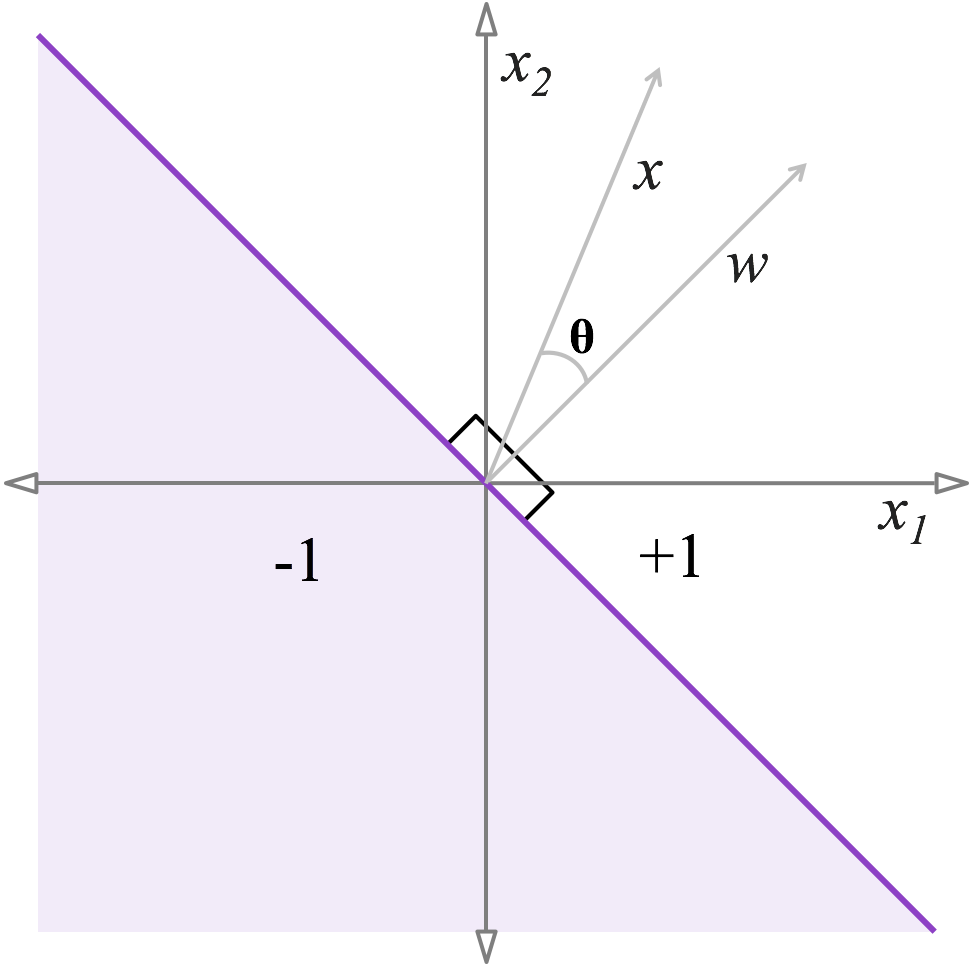
\includegraphics[height=0.45\textheight]{figures/linear-separator}
\par\end{center}

Suppose $\|w\|>0$ and $\|x\|>0$: 
\begin{eqnarray*}
f(x) & = & \left\langle w,x\right\rangle =\|w\|\|x\|\cos\theta\\
 f(x)>0 & \iff & \cos\theta>0 \iff\theta\in\left(-90^{\circ},90^{\circ}\right)\\
 f(x)<0 & \iff & \cos\theta<0 \iff\theta\not\in[-90^{\circ},90^{\circ}]
\end{eqnarray*}
 
\end{frame}

\begin{frame}
{Rewrite the scoring function}
\begin{itemize}
\item Remember that we want to scale to very large \# of classes and
reuse algorithms and analysis for binary classification
\begin{itemize}
\item $\implies$ a \textcolor{blue}{single weight vector} is desired
\end{itemize}

\item How to rewrite the equation such that we have one $w$ instead of $k$?
\pause
\begin{align}
w_i^Tx &= w^T\psi(x, i) \\
h_i(x) &= h(x, i)
\end{align}
\begin{itemize}
\item Encode labels in the feature space.
\item Score for each label $\rightarrow$ score for the ``\emph{compatibility}'' of a label and an input.
\end{itemize}
\end{itemize}
\end{frame}

\begin{frame}{The Multivector Construction}
How to construct the feature map $\psi$?
\pause
\begin{itemize}
\item What if we stack $w_{i}$'s together (\eg $x\in \bR^2, \sY = \pc{1,2,3}$)
\[
w=\left(\underbrace{-\frac{\sqrt{2}}{2},\frac{\sqrt{2}}{2}}_{w_{1}},\underbrace{0,1}_{w_{2}},\underbrace{\frac{\sqrt{2}}{2},\frac{\sqrt{2}}{2}}_{w_{3}}\right)
\]
\end{itemize}

\begin{itemize}
\item And then do the following: $\Psi:\reals^{2}\times\left\{ 1,2,3\right\} \to\reals^{6}$
defined by
\begin{eqnarray*}
\Psi(x,1) & := & \left(x_{1},x_{2},0,0,0,0\right)\\
\Psi(x,2) & := & \left(0,0,x_{1},x_{2},0,0\right)\\
\Psi(x,3) & := & \left(0,0,0,0,x_{1},x_{2}\right)
\end{eqnarray*}

\item Then $\left\langle w,\Psi(x,y)\right\rangle =\left\langle w_{y},x\right\rangle $,
which is what we want. 
\end{itemize}
\end{frame}


\begin{frame}
{Rewrite multiclass perceptron}
Multiclass perceptron using the multivector construction.

\begin{algorithm}[H]
	Given a multiclass dataset $\sD=\pc{(x, y)}$\;
	Initialize $w\leftarrow 0$\;
	\For{$\text{iter} = 1,2,\ldots,T$}{
	\For{$(x,y) \in \sD$}
 	{
 		$\hat{y} = \argmax_{y'\in \sY} w^T\psi(x, y')$ \tcp*[l]{Equivalent to $\argmax_{y'\in\sY} w_{y'}^Tx$}
 		\If(\tcp*[h]{We've made a mistake}){$\hat{y} \neq y$}{ 
 		$w \leftarrow w + \psi(x, y)$ \tcp*[l]{Move the scorer towards $\psi(x, y)$}
 		$w \leftarrow w - \psi(x, \hat{y})$ \tcp*[l]{Move the scorer away from $\psi(x, \hat{y})$}
 		}
  	}
  	}
\end{algorithm}
\textcolor{Green}{Exercise}: What is the base binary classification problem in multiclass perceptron?
\note{$w^T(\phi(x,i)-\phi(x,j)) > 0$.}
\end{frame}

%\begin{frame}
%    {\dis Geometric interpretation}
%\end{frame}

\begin{frame}
{Features}
Toy multiclass example: Part-of-speech classification
\begin{itemize}
\item $\cx=\left\{ \mbox{All possible words}\right\} $
\item $\cy=\left\{ \mbox{NOUN,VERB,ADJECTIVE,\ldots}\right\} $.
\note<1>{What are useful features?}
\pause{}
\item Features of $x\in\cx$: $\mbox{[The word itself], ENDS\_IN\_ly, ENDS\_IN\_ness, ...}$
\end{itemize}

How to construct the feature vector?
\begin{itemize}
\item Multivector construction: $w\in \bR^{d\times k}$---\textcolor{red}{doesn't scale}.
\pause
\item Directly design features for each class.
\begin{align}
\Psi(x,y)=\left(\psi_{1}(x,y),\psi_{2}(x,y),\psi_{3}(x,y),\ldots,\psi_{d}(x,y)\right)
\end{align}
\begin{itemize}
\item Size can be bounded by $d$.
\end{itemize}
\end{itemize}
\end{frame}

\begin{frame}
{Features}
Sample training data:
\begin{center}
\texttt{
The boy grabbed the apple and ran away quickly .
}
\end{center}
\pause

Feature:
\begin{eqnarray*}
\psi_{1}(x,y) & = & \ind{x=\mbox{apple AND }y=\mbox{NOUN}}\\
\psi_{2}(x,y) & = & \ind{x=\mbox{run AND }y=\mbox{NOUN}}\\
\psi_{3}(x,y) & = & \ind{x=\mbox{run AND }y=\mbox{VERB}}\\
\psi_{4}(x,y) & = & \ind{x\mbox{ ENDS\_IN\_ly AND \ensuremath{y=}ADVERB}}\\
\ldots
\end{eqnarray*}
\pause
\vspace{-2em}
\begin{itemize}[<+->]
\item E.g., $\Psi(x=\text{run},y=\text{NOUN})=\left(0,1,0,0,\ldots\right)$
\item After training, what's $w_{1},w_{2},w_{3},w_{4}$?
\item \textcolor{blue}{No need to include features unseen in training data}.
\end{itemize}

\end{frame}

\begin{frame}
{Feature templates: implementation}
\begin{itemize}
\item Flexible, \eg neighboring words, suffix/prefix.
\item ``Read off'' features from the training data.
\item Often sparse---efficient in practice, \eg NLP problems.
\item Can use a hash function: template $\rightarrow \pc{1, 2, \ldots, d}$.
\end{itemize}
\end{frame}

\begin{frame}
{Review}
Ingredients in multiclass classification:
\begin{itemize}
\item Scoring functions for each class (similar to ranking).
\item Represent labels in the input space $\implies$ single weight vector.
\end{itemize}
\pause

We've seen
\begin{itemize}
\item How to generalize the perceptron algorithm to multiclass setting.
\item Very simple idea. Was popular in NLP for structured prediction (\eg tagging, parsing).
\end{itemize}
\pause

Next,
\begin{itemize}
\item How to generalize SVM to the multiclass setting.
\item \think{Concept check}: Why might one prefer SVM / perceptron?
\note{Uniqueness of solution, online learning / efficiency, inductive bias (margin)}
\end{itemize}
\end{frame}

%================================== 


\subsection{Linear Multiclass SVM}
\subsubsection{Formulation through constraints on margin}

\begin{frame}{Margin for Multiclass}
\begin{description}
\item<1->[Binary]
\begin{itemize}
\item Margin for $(\xn, \yn)$:
\begin{align}
\yn w^T\xn
\end{align}
\item Want margin to be large and positive ($w^T\xn$ has same sign as $\yn$)
\end{itemize}

\item<2->[Multiclass]
\begin{itemize}
\item Class-specific margin for $(\xn, \yn)$:
\begin{align}
h(\xn,\yn)-h(\xn,y).
\end{align}
\item Difference between scores of the correct class and each other class
\item Want margin to be large and positive for all $y\neq \yn$. 
\end{itemize}
\end{description}
\end{frame}
%

\begin{frame}
{Multiclass SVM: separable case}
\begin{description}
\item<1->[Binary] 
\begin{align}
\min_w \quad & \frac{1}{2}\|w\|^2 \\
\text{s.t.} \quad& \underbrace{\yn w^T\xn}_{\text{margin}} \geq 1 \quad \forall (\xn, \yn) \in \sD
\end{align}

\item<2->[Multiclass] As in the binary case, take 1 as our target margin.
\begin{align}
m_{n,y}(w)&\eqdef \underbrace{\left\langle w,\Psi(\xn,\yn)\right\rangle}_{\text{score of correct class}}
- \underbrace{\left\langle w,\Psi(\xn,y)\right\rangle}_{\text{score of other class}} \\
\min_w \quad & \frac{1}{2}\|w\|^2 \\
\text{s.t.} \quad& m_{n,y}(w) \geq 1 \quad
\forall (\xn, \yn) \in \sD,\, y\neq \yn
\end{align}

\end{description}
\onslide<3->{
\think{Exercise}: write the objective for the non-separable case
}
\note<3->{Next, let's think about how to write the objective using hinge loss.}
\end{frame}

\subsubsection{Formulation through hinge loss}
\begin{frame}
{Recap: hingle loss for binary classification}
\begin{itemize}
\item Hinge loss: a convex upperbound on the 0-1 loss
\begin{align}
\ell_{\text{hinge}}(y, \hat{y}) = \max(0, 1 -  yh(x))
\end{align}
\begin{figure}
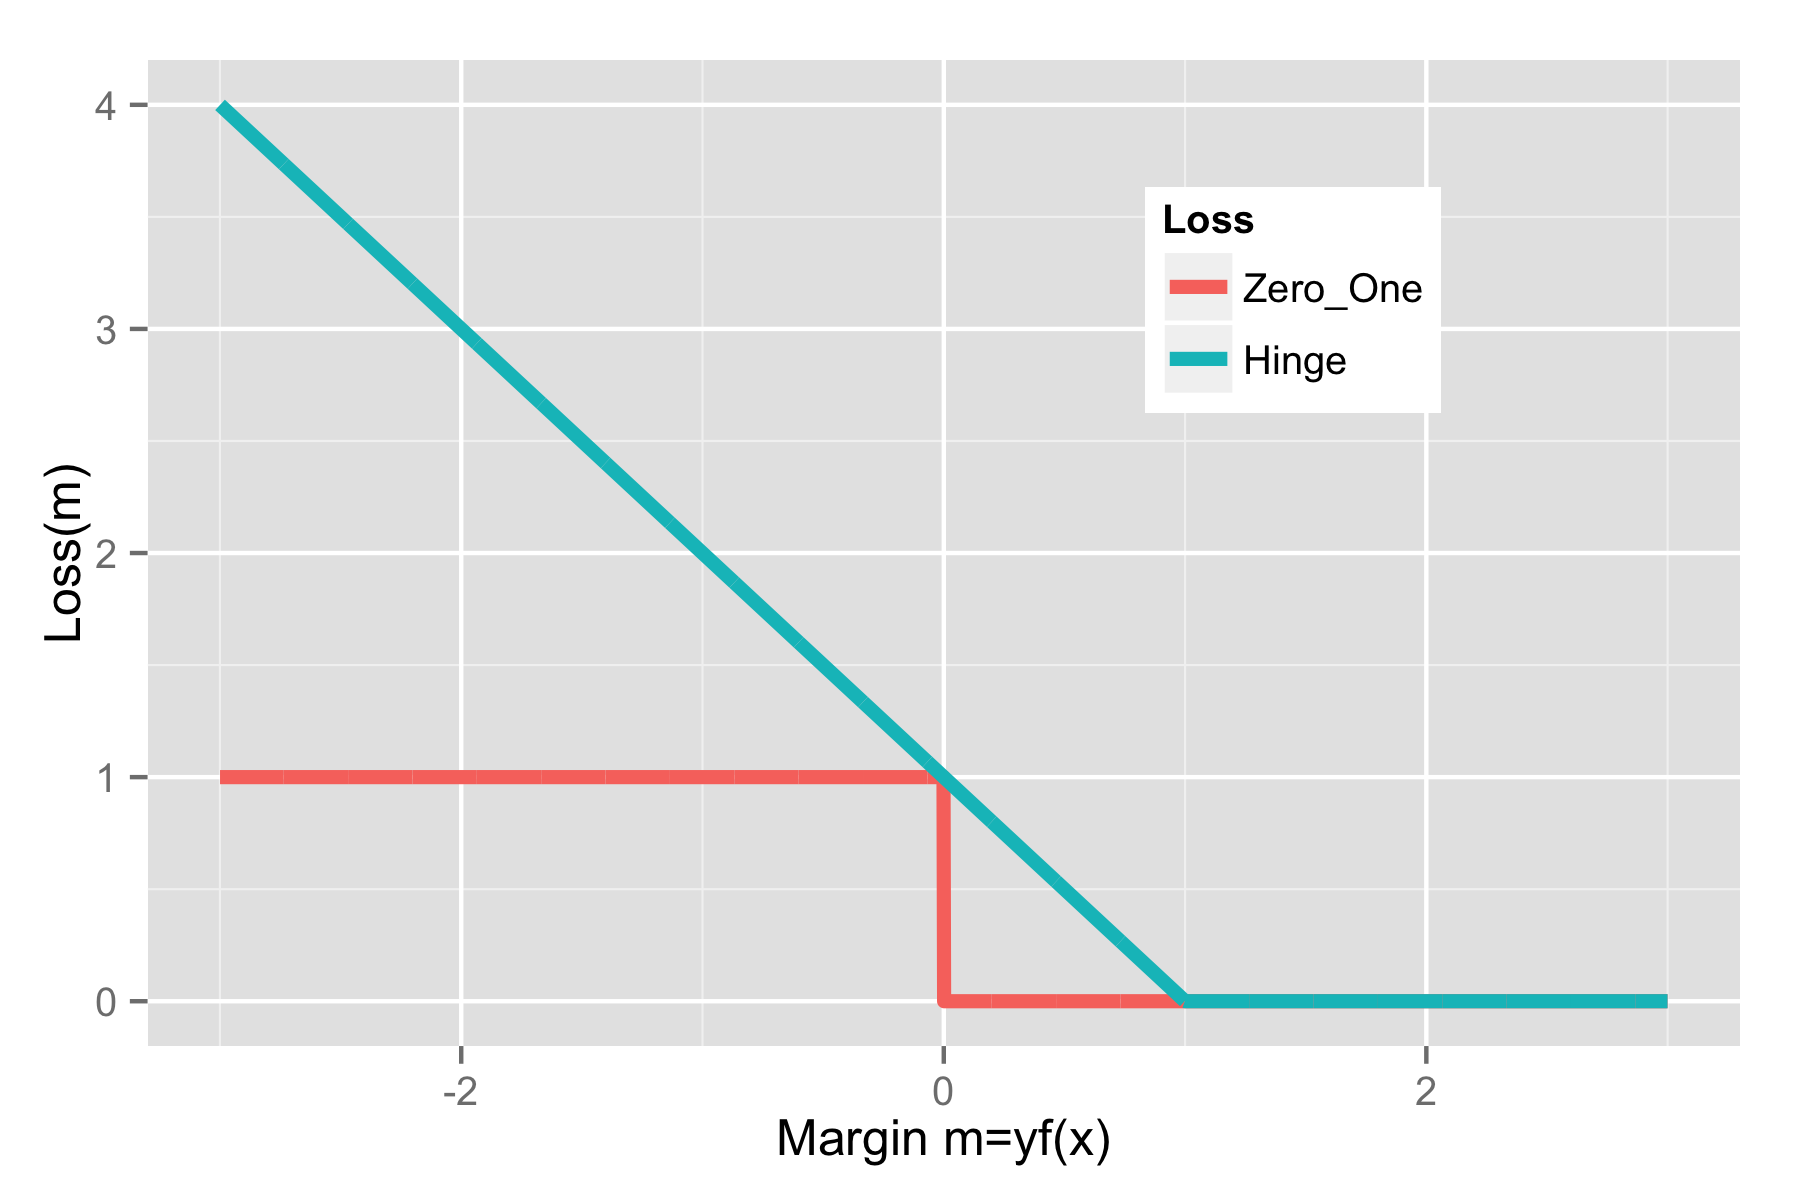
\includegraphics[height=0.5\textheight]{{figures/loss.Zero_One.Hinge}.png}
\end{figure}
\end{itemize}
\end{frame}

\begin{frame}
{\dis Generalized hinge loss}
\begin{itemize}[<+->]
\item What's the zero-one loss for multiclass classification?
\begin{align}
\onslide<+->{\Delta(y, y') = \1\pc{y\neq y'}}
\end{align}
\item In general, can also have different cost for each class.

\item Upper bound on $\Delta(y, y')$.
\begin{align}
\hat{y} &\eqdef \argmax_{y'\in\sY} \left\langle w, \Psi(x, y') \right\rangle \\
\onslide<+->{
\implies & \left\langle w, \Psi(x, y) \right\rangle \leq
\left\langle w, \Psi(x, \hat{y}) \right\rangle \\
}
\onslide<+->{
\implies & \Delta(y, \hat{y}) \leq \Delta(y, \hat{y}) -
\left\langle w, \p{\Psi(x, {y}) - \Psi(x, \hat{y}}) \right\rangle
&& \text{When are they equal?}
}
\end{align}

\item Generalized hinge loss:
\begin{align}
\ell_\text{hinge}(y, x, w) \eqdef
\max_{y'\in\sY}\p{
\Delta(y, {y'}) -
\left\langle w, \p{\Psi(x, {y}) - \Psi(x, {y'}}) \right\rangle
}
\end{align}
\note<+->{When $y'=y$, $\ell_{\text{hinge}}=0$.}
\end{itemize}
\end{frame}

\begin{frame}{Multiclass SVM with Hinge Loss}
 
\begin{itemize}
\item Recall the hinge loss formulation for binary SVM (without the bias term):
\[
\min_{w\in\reals^{d}}\frac{1}{2}||w||^{2}+C\sum_{n=1}^{N}\max\left(0,1-\underbrace{\yn w^{T}\xn}_{\text{margin}}\right).
\]

\pause{}
\item The multiclass objective: 
\[
\min_{w\in\reals^{d}}\frac{1}{2}||w||^{2}+
C\sum_{n=1}^{N}\max_{y'\in\sY} \p{
\Delta(y, {y'}) -
\underbrace{
\left\langle w, \p{\Psi(x, {y}) - \Psi(x, {y'}}) \right\rangle
}_{\text{margin}}
}
\]

\begin{itemize}
\item $\Delta(y, y')$ as \textcolor{blue}{target margin} for each class.
\item If margin $m_{n, y'}(w)$ meets or exceeds its target $\Delta(\yn,y')$
$\forall y\in \sY$, then no loss on example $n$. 
\note<2->{If exceeds margin, loss is negative, which must be smaller than loss of the true class, which is zero.}
\end{itemize}
\end{itemize}
\end{frame}
%

\subsection{Is This Worth The Hassle Compared to One-vs-All?}
\begin{frame}{Recap: What Have We Got?}
\begin{itemize}
\item Problem: Multiclass classification $\cy=\left\{ 1,\ldots,k\right\} $
\end{itemize}

\pause{}
\begin{itemize}
\item Solution 1: One-vs-All


\begin{itemize}
\item Train $k$ models: $h_{1}(x),\ldots,h_{k}(x):\cx\to\reals$.


\item Predict with $\argmax_{y\in\cy}h_{y}(x)$.


\item Gave simple example where this fails for linear classifiers
\end{itemize}
\end{itemize}

\pause{}
\begin{itemize}
\item Solution 2: Multiclass loss


\begin{itemize}
\item Train one model: $h(x,y):\cx\times\cy\to\reals$.


\item Prediction involves solving $\argmax_{y\in\cy}h(x,y)$.
\end{itemize}
\end{itemize}
\end{frame}
%
\begin{frame}{Does it work better in practice?}
\begin{itemize}
\item Paper by Rifkin \& Klautau: ``\href{http://www.jmlr.org/papers/v5/rifkin04a.html}{In Defense of One-Vs-All Classification}''
(2004)
\begin{itemize}
\item Extensive experiments, carefully done 
\begin{itemize}
\item albeit on relatively small UCI datasets
\end{itemize}
\end{itemize}


\begin{itemize}
\item Suggests one-vs-all works just as well in practice
\begin{itemize}
\item (or at least, the advantages claimed by earlier papers for multiclass
methods were not compelling)
\end{itemize}
\end{itemize}
\end{itemize}

\pause
\begin{itemize}
\item Compared 
\begin{itemize}
\item many multiclass frameworks (including the one we discuss)
\item one-vs-all for SVMs with RBF kernel
\item one-vs-all for square loss with RBF kernel (for classification!) 
\end{itemize}
\end{itemize}


\begin{itemize}
\item All performed roughly the same
\end{itemize}
\end{frame}
%
\begin{frame}{Why Are We Bothering with Multiclass?}
\begin{itemize}
\item The framework we have developed for multiclass
\begin{itemize}
\item compatibility features / scoring functions
\item multiclass margin
\item target margin / multiclass loss
\end{itemize}
\end{itemize}

\pause{}
\begin{itemize}
\item Generalizes to situations where \textcolor{blue}{$k$ is very large} and one-vs-all
is intractable.
\end{itemize}

\pause{}
\begin{itemize}
\item Key idea is that we can \textcolor{blue}{generalize across outputs $y$ by using features
of $y$}.
\end{itemize}
\end{frame}

\end{document}
